\documentclass[titlepage]{article}
\usepackage{hyperref}
\usepackage{graphicx}
\graphicspath{ {../Diagrams/} }

% Title Page
\title{Real-time Trading Platform - Interim Report}
\author{John Costa - 100943301}
\date{06 Oct 2022 \\
  \\
  \Large{Final Year Project \\
Supervised By: Julien Lague \\
Royal Holloway, University of London}}

\begin{document}
\maketitle

\section{Introduction}
\subsection{The Problem}
For my final year project, I am creating a Real-time Trading platform, with a web interface and a robust backend, allowing the many users of the platform to trade - in real-time - with each other, with very low latency.

\subsection{Aims and Goals}
- Low latency
- Scalable
- Distributed
- Complex user actions on web interface
- Learn about it


\subsection{Research}
My primary source of information is the book \textit{Desining Data Intensive Application} ~\cite{kleppmann_2021}. This book provides an array of knowledge about building data intensive distributed applicatios that are reliable, scalable and usable.

\subsection{Objectives}
- Authentication
- Allow users to buy/sell assets
- Scale

Currently I have authentication working, I also have the basic features of allowing users to buy and sell pre-set assets on the platform. I have called this stage the PoC (Proof of concept), where I built the basic features, to get a solid, working foundation - but also because it only includes a subset of the features, I was able to build it fairly quickly and fail very quickly. Furthermore it made me learn.

\section{Architecture}
One of my projects main goals is to have a scalable architecture, which can automatically scale depending on load from the end users, I needed to create a robust architecture, by splitting the project into smaller systems which all work and communicate together. The advantage of this is that I am able to individually scale each system, without affecting or needing to scale the others, giving me much finer control over this property of the project. \\

My project is split into the following (micro) services:
\begin{itemize}
  \item Authentication - User authentication.
  \item Hub - Initial point of contact for users.
  \item Brain - Permanent storage and data management.
\end{itemize}

Each of these services has their own database, as to reduce the dependency on a shared database. Below I go into further detail on each of these systems, I have also included a system diagram.

\hspace*{-3cm}
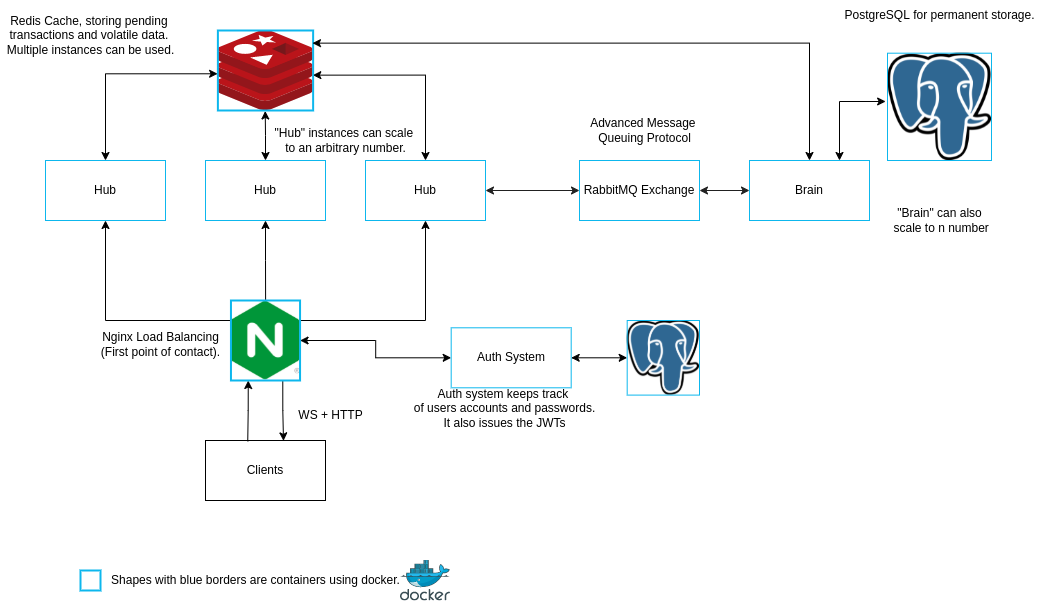
\includegraphics[width=1.5\textwidth]{Architecture.png}

\subsection{Authentication}
This system is the most isolated from the others. As you can see on the diagram is only communicates with the load balancer which comes straight from the user. This is because communication to and from the auth system contains very secure information such as passwords and access tokens, which if intercepted can allow users to access another users account. Therefore I don't want to handle this information for longer than I need to and definetly through the least number of systems possible - like this we go from the user to Nginx (A load balancer), straight to my authentication system. \\

The authentication system has its own database with a few tables that store user information. The database I choose is PostgreSQL, which as outlined in my plan, is one of the fastest, most robust and safest permaennt storage databases in the world, often outperforming competition by magnitudes or performance. The tables for this database are as follows: \\

TODO: Figure out how to make these nice
\begin{itemize}
  \item users
  \item userlogs
\end{itemize}

it includes 3 methods, and uses JWT, etc...

\subsection{Hub}
The hub is the only service without any permanent storage and this is very intentional. Its job is to act as a router for other services, but also a cache. My aim is to have this service serve from cache around 50 percent of the time. The hub communicates with a redis database which is a key pair in-memory database, which acts as a very fast caching system, that stores frequently requested data, as to avoid requesting this data from other systems. \\

The Hub can be vertically scaled very easily, together with the Redis database that it users, as Redis supports vertical scaling in a cluster mode. It is likely the system that will be scaled the most, as it will handle all of the users request (except for authentication).

\subsection{Brain}
A terrible name, but the Brain performs CRUD operations on the assets and transactions for the entire system, it acts as an API which the Hub can communicate with to fetch information from. The Brain like all other services has a database of its own, another PostgreSQL database. The Brain can also scale vertically just like all services but it's difficult to scale the PostgreSQL database vertically because it is difficult to split the data, instead a horizontal scaling approach will be required for the database portion of this service. \\

The brain also communicates with the Redis cluster which the Hub primarily interacts with. This is to update the cache so that the Hub can in future requests return data from this cache database instead of requesting the data from the Brain. The reason I do this step in the Brain service instead of on the Hub on return of the data, is because I want the Hub to only be conserned with handling user requests and either returning the data from cache, or handing it off to another service, as to not "Hold up the line". TODO: JUSTIFY THIS DECISONI WITH THE BOOK AND RESEARCH.

\subsection{Communication and Loadbalancing}
I have not yet described how these systems communicate with either one another or the user. To start with the user makes request to Nginx which can act as a very high performance web server, load balancer or reverse proxy. These requests are HTTP(s) requests (and also WS), and therefore this is what the Hub recieves from the user. \\

However, for the hub to communicate with the Brain service it does not use HTTP requests as these would be somewhat inefficient and not complex enough to handle some of the required distributed behavior of the systems, therefore I am using RabbitMQ to commuinicate between the Brain service and the Hub. RabbitMQ acts as a message exchange which supports AMQP (Advanced Messaging Queue Protocol), and with this I can create a sort of RPC (Remote Prodedural Call), from the Brain service. All whilst allowing many messages from multiple isntances of both services. \\

\section{Technologies used}
I have a variety of technologies for my project, these include frontend technologies to create a state of the art web interface, to backend technologies that allow the project to be scaled to as many users as it needs to be scaled to. \\

I have already talked about some of the technologies used. TODO: REFACTOR.

\subsection{Backend Technologies}
These are the technologies which I used to build the backend system, which consists of the Hub, Brain and Authentication. \\

\subsubsection{Golang}
As a programming language I have used Golang TODO: INSERT REF, it is a statically typed compiled language, known for its simplicity and ability to write extremely scalable systems, doing my own research I have found that a lot of modern architectures use Golang Real-time Trading Platform
John Costa - 100943301
06 Oct 2022
CS3821 - BSc Final Year Project
Supervised By: Julien Lague
Royal Holloway, University of Londonbecause of its stuff TODO: ADD REFS AND EXAND. \\

Golang also has an extremely fast compiler.

\subsubsection{PostgreSQL}
PostgreSQL is a relational database written in C, known for its performance and reliality. It uses SQL (Strucutured Query Language), to allow users to interact with the database. I have outlined the reason The reason I choose this database is because it consistently outperforms other databases (Both relational and non-relational), and performance is extremely important when building a system such as this one. However PostgreSQL does have limitation, such that it can only (easily), scale horizontally (Increasing the size of the machine), this is mostly due because the data is very centralized and highly linked in a relational database, but even with this big drawback, it still is the best, most performant option. To mitigate this drawback I have split the databases across the services, as to not have 1 central database, which would have been easier but would create a performance bottleneck. TODO: LOOK IN BOOK FOR REF.

\subsubsection{Redis}
Redis is an unstructured key-value pair in-memory database. Because it is in-memory, it is magnitudes faster than any persistent storage database, therefore I have used it as caching in my system, storing popular assets and data that is used frequently. \\
However, it is important that all the data stored in Redis, can be lost. This means I first have to store it in permanent storage, and only then store it for use in Redis. \\

The need for caching is extremely important in these systems. TODO: Further research on this.

\subsubsection{Docker}
Docker is an engine for running docker containers, a very barebones VM which doesn't contain an OS and relies on the OS of the host machine, because of this Docker containers are very quick to spin up and down, and are much more lightweight than a full VM. I have used docker to run all of the systems on my system, allowing me to very quickly spin up more instances of these systems or reduce the amount of others depending on load. \\

To manage the complexity of running many docker containers I have used Docker Compose TODO: REF. This is a way to describe your architecture in a YAML file and run the 1 file, which takes care of all configuration. Not only is this used in production, it is also used during development to spin up all the backend systems needed when I am developing. \\

Furthermore, Docker can be ran in what is called Docker Swarm. This is a way to keep multiple instances of the same system, increase the amount of replicas or decrease them based on load. This is very useful as my system needs to scale. \\

\\
\noindent
{\large Why not use Kubernetes?} \\
\\
Too complicated, and definetly overkill.

\subsubsection{RabbitMQ}
TODO: RESEARCH ON MESSAGING SYSTEMS

\subsubsection{Nginx}
Nginx has multile functions. It can act as a load balancer, a web server and a reverse proxy. All of which my system will use. Nginx is very performant, easily handling 1000s of requests a second, with its event-based architecture, it is trusted my most companies to be the gateway into their systems. In my case all of the users requests will go into Nginx to be load balanced across multiple instances of the Hub service. I am also going to use Nginx to statically serve the files for the frontend application.

\subsubsection{Gin - Golang HTTP Server}
A nice framework for building APIs using go.

\subsubsection{JWT}
JSON Web Tockets or JWTs for short, are cryptographically safe methods of client side authentication. A JWT is generated in the Authentication system, and signed with a private key, everytime the user wishes to authenticate themselves, they serve the JWT to any system, and if the signature on the JWT is correct then the user is authenticated, if not, we know the user either tampered with the signature or it isn't a valid JWT. JWTs can only encode a small amount of data in them, ranging from user information and ids, however this information is assessible to anyone who views the JWT, so it is important that the data is public knowledge. \\

I choose to use JWTs instead of cookie because they are very safe but still quite practicle. Like this I do not need to store cookies in the database and check everytime against a database that the user is logged in, reducing the amount of lookups various systems would have to perform.

\subsection{Frontend technologies}
Making a website is very hard now a days.

\subsubsection{SolidJS}

\subsubsection{Vite}

\subsubsection{Websockets}

\section{Software Engineering}

\subsection{Methodology}

\subsection{Version Control}

\subsubsection{Monorepo}
For this project, we were provided with 1 GitLab repo, however my project consists of various different services and parts that normally would not belong in the same repo. However, there is a common technique in industry of keeping all your code base in the same repository (monorepo), hence making CI (Contant Integration) and development easy, because everything is in one place and not scattered across multiple different project repositories. I am not using any monorepo management software although these do exist (Turborepo, Monorepo, Bazel), I keep my different projects stored in the apps TODO: Add formatting direcotry, hence seperating these somewhat, and each apps configuration files are stored in their corresponding folder, leaving the overall structure of the repository nice and clean.

\subsubsection{Bare repo and Worktrees}
Git has a feature called worktrees, this feature is not very well known, however I think it is a very powerful feature and one I have used through this project. Starting with cloning a barerepo, this means that we clone a Git Repository without cloning any of the files in the folder, with the main branch checked out. However, a bare clone just clones the .git file withotu any of the files, and we can use worktrees to edit various branches, worktrees are a way to have multiple branches in a git repository checked out at the same time, in seperate folders. This feature is very powerful because I was often working on 2 things at the same time (Frontend, backend and maybe the report), and naturally these live in different branches, therefore it is extremely useful to have them all checkout out at the same time. TODO: ADD REFERENCE FOR WORKTREES.

\subsection{Testing}

\subsection{Documentation}

\section{Assessment}

\bibliography{ref}
\bibliographystyle{plain}

\end{document}
